\subsubsection{Secure Element} \label{section:counter-replace-encryption-key-local}
Since there is the possibility to read the cached encryption key \cite{memoryDump} and crack the encryption, the use of \gls{se} is proposed.
A secure element is a tamper-resistant platform which can be used to securely host applications and cryptographic keys \cite{seDefinition}.
There are different form factors for \gls{se}s.
For Android, the microSD form factor is the interesting one.
It can be either mounted in the SD Card slot or by using an adapter on the USB interface, which requires the device to support \gls{otg} \cite{usbOtg}.
The resource is accessed over reads and writes to the filesystem.
Since the \gls{se} has to be small to fit the size of an SD Card and powered by the host system, its hardware capabilities are constrained.
The result is a performance of 25MHz which does not allow complexe comnputations. \cite{stSe}
\newline
For this reason the usage of the \gls{se} is restricted to simple tasks, like storing a key used for decryption.
The advantage of an \gls{se} is that its functionality is outside of the Android application and thus cannot be manipulated by \gls{luckypatcherg}.
\newline
An abstract presentation of the use of a \gls{se} can be seen in figure~\ref{fig:encryptionKeySmart}.
\newline
\begin{figure}[h]
    \centering
    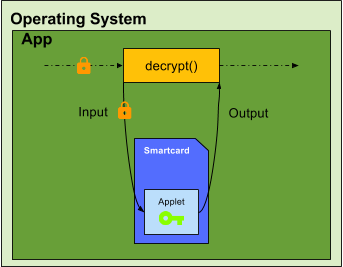
\includegraphics[width=0.8\textwidth]{data/encryptionKeySmart.png}
    \caption{Decryption by using a smartcard}
    \label{fig:encryptionKeySmart}
\end{figure}
Integrating a \gls{se} comes with some problems.
\begin{itemize}
  \item the user has to buy extra hardware
  \item not all devices have a SD Card slot or support \gls{otg}
  \item different implementations for communication with the \gls{se}
\end{itemize}



same as internet service but extra hardare has to be bought
people are lazy and do not want to have extra hardware
when integrated into phone, it will take a long time until each phone supports it, e.g. was not able to use it on Nexus 6P and Nexus 7, Linux did not recognize it but mass storage was enabled, Nexus7 said OTG available but it did not work
many different implementation fragmentate the market, there is not one single solution to focus on and push for market wide accepted solution
solution which are out there have major security flaws, smartcard itself can be attacked

have problems on their own, nur so sicher wie das secure element
DAP Verification .... normalerweise muss jede Applet, die auf so ein Secure Element/Smartcard etc. kommt mit ner Signatur unterschrieben sein ...
%\url{http://www.win.tue.nl/pinpasjc/docs/Card%20Spec%20v2.1.1%20v0303.pdf}


Waehrend ich Exploits finden konnte, die Dir erw. Zugriff geben, wenn du Applets installieren kannst, u.a.
%\url{https://www.cs.ru.nl/E.Poll/papers/cardis08.pdf}
%\url{http://www.uclouvain.be/crypto/wissec2009/static/13.pdf}​

SD Association
\url{http://www.androidpolice.com/2016/02/22/with-smartsd-the-sd-association-wants-to-adapt-microsd-cards-to-make-mobile-payments/}





TODO:
2) Secure Elements
Bottleneck ist sicherlich die Schnittstelle zu Android und alles was in Android ist, ist prinzipiell unsicher, also auch etwaige Keys. Was jedoch koennte Secure Elements absichern? Ich moechte dich bitten hier Ideen zu erarbeiten, was im Zuge von Kopierschutz,  Verschluesslung etc. mit SEs wirklich sicher gemacht werden koennte. Eine grobe Idee ist z.B. das Signieren von Serveranfragen. Key kennt hier nur das SE und der Server. Android schickt die volle URL mit Parametern und das SE fuegt einen Signaturparameter zu. Vorteil: Ohne das SE kann die App den Server mal nicht mehr nutzen. Jetzt musste man verhindern, dass eine Proxy-App unter Android fuer andere aktiv wird (Stichwort CardSharing). Was koennte man tun? Das ist auch nur ein Idee. Was gibt es sonst noch? Wo koennte es Sinn machen einen sicheren Speicher zu haben?
